\section{局部多项式曲面构造}
% \noindent{\parbox{\textwidth}{{\wn{Question:}
%       几阶的多项式曲面可以使得界面追踪精度达到4阶?}}}
% \noindent{\fbox{\parbox{\textwidth}{{\wn{Question:}
%        几阶的多项式曲面可以使得界面追踪精度达到4阶?
%        \uline{u*}}}}}
 % \begin{itemize}
 % \item 推广一元多项式插值余项的推导方式?
 %   ($\mathrm{R}^m\rightarrow \mathrm{R}^n的Roller's Theorem$)
 % \item 参考张量曲面的误差分析
 % \item 转化成点在曲线上分析?
 % \end{itemize}
\begin{rem}
  由于我们用于追踪流体界面的点在空间上是散乱分布的,
  而且已经有三角剖分的结构,因此我们考虑基于三角剖分的二维样条函数。
\end{rem}
\subsection{Bernstein 基多项式}
%%%%%%%%%%%%%%%%%%%%%%%%%%%%% Constants
% a.向前追踪边界上的示踪点b.如果下一时刻的三角性边长大于$h_L$,
% 回溯原来的三角形,在原来的三角形边长中增加中点对应的插值曲面上的点作为新的示踪点

%  插值曲面的构造。

% 将三角网格点投影在x-y平面,向外找star上的示踪点投影到x-y平面。
% 如果一层star没有合适的十个点就向外再裹一层。

% 取最外面的三个点构成包裹的三角形T,
% 运用三角形的重心坐标和Bernstein basis polynomials of degree d relative
% to T,
\begin{nota}
  $d$阶多项式空间
  \begin{displaymath}
{\cal P}_d:=\left\{ p(x,y) = \sum_{0\leq i+j\leq d}c_{ij}x^iy^j\right\}.
  \end{displaymath}
\end{nota}
\begin{defn}
  给定整数$d>0$,和三角形$T$相关的$d$阶 Bernstein 基多项式定义为
  \begin{displaymath}
    B^d_{ijk}:=\frac{d!}{i!j!k!}b^i_1b_2^jb_3^k,\quad i+j+k=d,
  \end{displaymath}
  $i,j,k$是非负整数。
\end{defn}
\begin{prop}
  Bernstein基多项式性质:
  \begin{enumerate}
  \item $ 0\leq B_{ijk}^d(x,y)\leq 1 \quad (x,y) \in T,$
  \item $ \sum_{i+j+k=d}B_{ijk}^d(x,y) \equiv 1\quad (x,y)\in T.$
  \end{enumerate}
\end{prop}


\begin{lem}
  多项式 $\left\{ B^d_{ijk}\right\}$线性独立,
  且构成$d$次多项式${\cal P}_d$线性空间的一组基,维数是
  $\begin{pmatrix}
    d+2\\ 2
  \end{pmatrix}$。
\end{lem}

% \begin{nota}
%   ${\cal S}^0_d(\triangle):=\{s\in C^0(\Omega):s|_{T_i}\in{\cal P}_d ,
%   \quad i=1,...,n_t\}.$
% \end{nota}
% \begin{prop}  \begin{displaymath}
% \textmd{dim} {\cal S}^0_d(\triangle)=n_v+(d-1)n_e+\frac{(d-1)(d-2)}{2}n_t,
% \end{displaymath}
% 其中,$n_v,n_e$和$n_t$分别是三角剖分的点、边和三角形个数。
% \end{prop}

\begin{rem}
  为了达到四阶精度,我们用$p\in {\cal P}_3$
  \begin{displaymath}
    p(x,y)=\sum_{i+j+k=3}c_{ijk}B_{ijk}^d=\sum_{i=1}^{10}c_iB_i,
  \end{displaymath}
  其中$c_i,1\leq i\leq 10$分别
  是
  $c_{300},c_{210},c_{201},c_{120},c_{111},c_{102},c_{030},c_{021},c_{012}$,
  $c_{003}$.
\end{rem}



\begin{rem}
  考虑以下两种局部曲面表示
  \begin{enumerate}
  \item 基于适定结点组生成算法的局部二元三次多项式插值\cite{ShaoThesis};
  \item 基于三角剖分的局部部分插值部分最小二乘拟合
    \cite{schumaker2015spline}.
  \end{enumerate}
\end{rem}

\subsection{基于三角剖分的局部部分插值部分最小二乘拟合}
\label{sec:局部三次样条曲面}
\begin{defn}[算法]\cite{schumaker2015spline}
  对于任意的三角剖分中的三角形,
\begin{enumerate}
\item 以三角形为中心,寻找合适的拟合点。
  取三个顶点star中的所有点。
  如果点大于20,取距离三角形中心最近的20个点。
\item 根据在三个三角形顶点插值,最小二乘拟合其他点的条件,
  计算三次样条基函数的系数。
\end{enumerate}
\end{defn}

\begin{lem}
  设三角形$T$ 的三个顶点分别是$v_1,v_2$ 和 $v_3$.
 给定点列 $\{p:=(x_i,y_i)^m_{i=1}\}$对应的值 $\{z_i\}^m_{i=1}$
 令
  \begin{displaymath}
    O:=[B_1(p_j),...,B_{10}(p_j)]_{j=1}^m,
  \end{displaymath}
  其中$B_1,...,B_{10}$是关于$T$的三次Bernstein基多项式。
  令$\tilde{O}$是$O$去掉第1,7,10列的子矩阵,且满秩。
  则对任意的$\{\omega_i\}_{i=1}^3$,存在一个唯一的二元三次多项式使得
  \begin{displaymath}
    g:=\sum_{i=1}^{10}c_iB_i
  \end{displaymath}
  满足$g(v_i)=w_i,i=1,2,3$,且极小化
  \begin{displaymath}
    \sum_{j=1}^m[g(p_j)-z_j]^2.
  \end{displaymath}
\end{lem}

\begin{pro}
  由Bernstein基多项式的性质可以通过令$c_1 = w_1, c_7 = w_2, c_{10} = w_3$确保$g(v_i)=w_i,i=1,2,3$。
  \begin{displaymath}
    \boldsymbol{c} = \left[
      \begin{matrix}
        c_2\\
        \vdots\\
        c_6\\
        c_8\\
        c_9
      \end{matrix}
    \right], 
    \boldsymbol{b} = \left[
      \begin{matrix}
        z_1\\
        \vdots\\
        z_m
      \end{matrix}
    \right] - w_1O_1-w_2O_7-w_3O_{10}.      
  \end{displaymath}
  为了得到其余的多项式,求解超定方程组
  \begin{displaymath}
    \tilde{O}\boldsymbol{c} = \boldsymbol{b}
  \end{displaymath}
  由于$\tilde{O}$列满秩,等价于求解正规方程
  \begin{displaymath}
    \tilde{O}^T\tilde{O}\boldsymbol{c} = \tilde{O}^T\boldsymbol{b}.
  \end{displaymath}
  得到唯一的最小二乘解。
\end{pro}

\subsection{数值测试结果}

\begin{figure}[H]
  \centering
  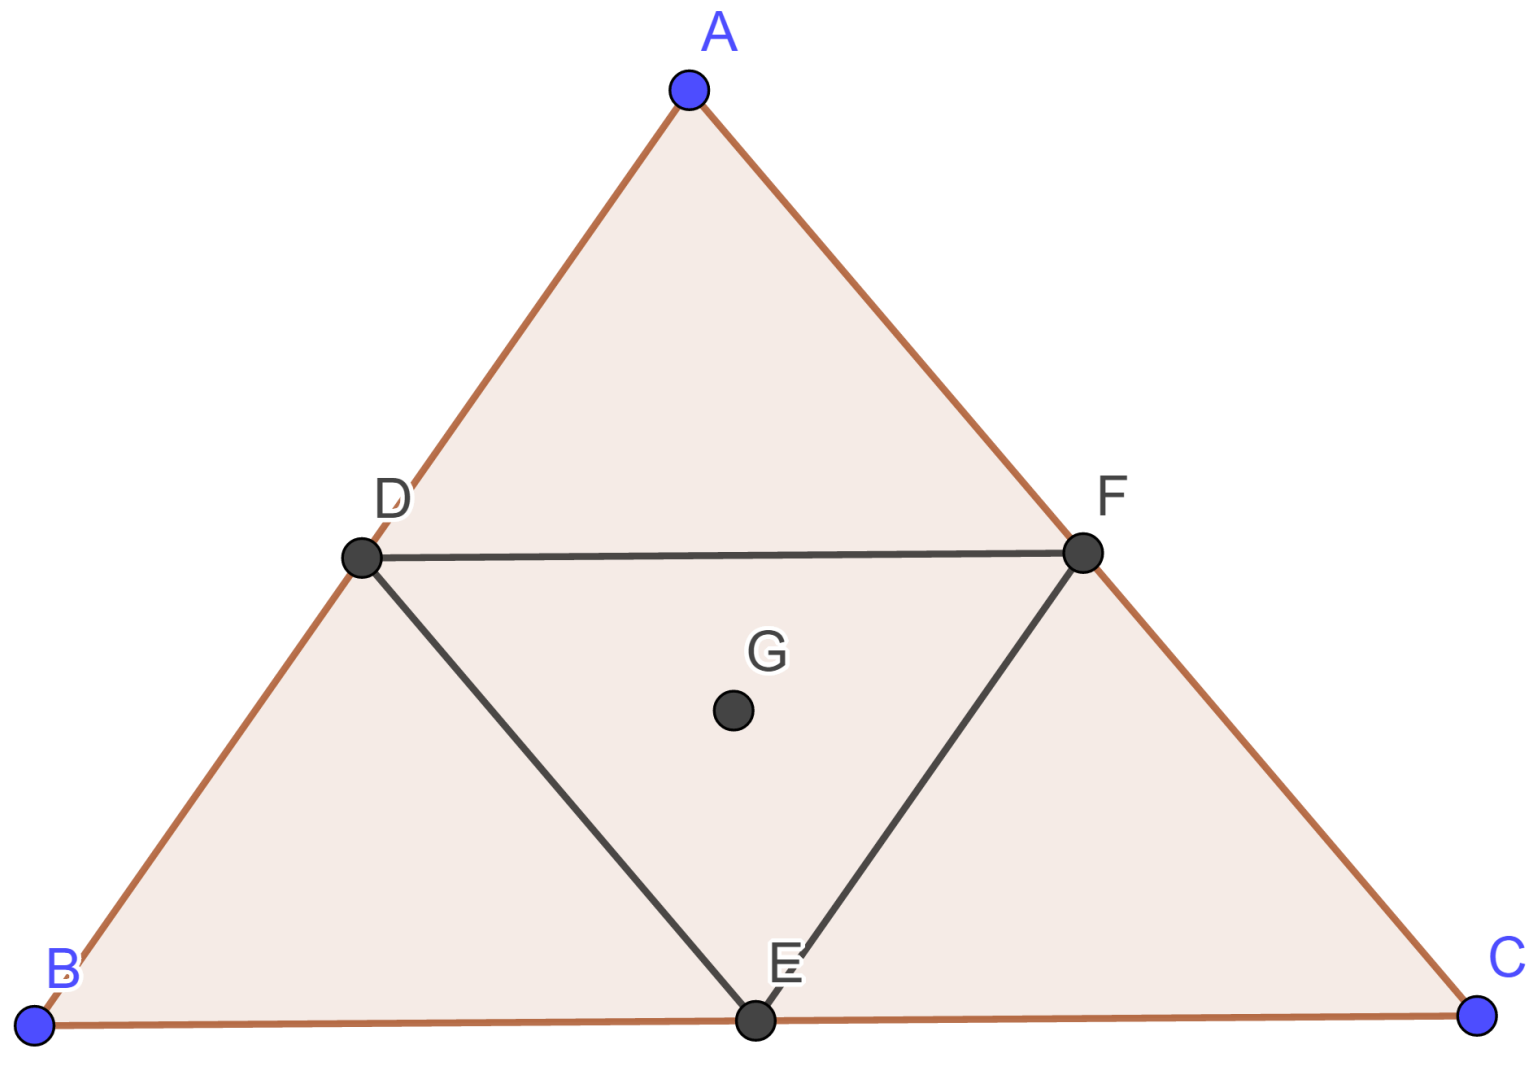
\includegraphics[width=0.35\linewidth]{images/tri}
  \caption{加密网格的方法}
\end{figure}
\begin{table}[htbp]
  \begin{center}  
    \begin{tabular}{|l|l|l|l|l|l|l|l|}  
      \hline  
      norm & $|E_h|$ & rate & $|E_{h/2}|$ & rate& $|E_{h/4}|$ &rate &$|E_{h/8}|$ \\
      \hline            
      1-norm & 2.77e-3 & 3.09 & 3.25e-4 & 4.34& 1.60e-5 & 3.89&1.07e-6 \\
      \hline
      2-norm & 5.97e-4 & 3.56 & 5.05e-5 & 4.00& 3.15e-6 & 4.82&1.11e-7 \\
      % 5 & 2.11e-3 & 8.12 & 3.28e-3 & -& 9.88e-06 \\  \hline
      \hline  
    \end{tabular}  
  \end{center}  
  \caption{局部完全插值}  
\end{table}
\begin{table}[h]
  \centering
  \begin{tabular}{|c|c|c|c|c|c|c|}
    \hline
    $|E_h|$ & rate & $|E_{h/2}|$ & rate& $|E_{h/4}|$&rate&$|E_{h/8}|$\\ 
    \hline
    1.74e-5& 5.19& 4.77e-7& 5.10& 1.38e-8& 4.03& 8.48e-10\\ 
    \hline
  \end{tabular}
  \caption{局部部分插值结合最小二乘}
\end{table}
